\section{Multiplicador de Voltaje}

    Debido a que el sensor de corriente y el DAC diseñados necesitan una
    alimentación simétrica de $\pm 7\text{V}$ (como mínimo), se diseñó 
    un multiplicador de voltaje basado en el circuito \textit{negative 
    Dickson charge pump} presentado en la sección \ref{sec:charge_pump}.


    Puesto que este necesita de una señal cuadrada, se utilizó un inversor
    elaborado con un transistor BJT , en cascada con una etapa de salida 
    \textit{push-pull}. El inversor es empleado para generar una señal
    cuadrada de amplitud $12\text{V}$ a partir de una señal cuadrada 
    de $5\text{V}$, mientras que la etapa \textit{push-pull}
    es utilizada para aumentar la corriente de salida del inversor, de forma
    que sea capaz de alimentar el multiplicador de voltaje. El circuito
    se muestra en la figura \ref{fig:inversor}.
    
    \begin{figure}[H]
        \centering
        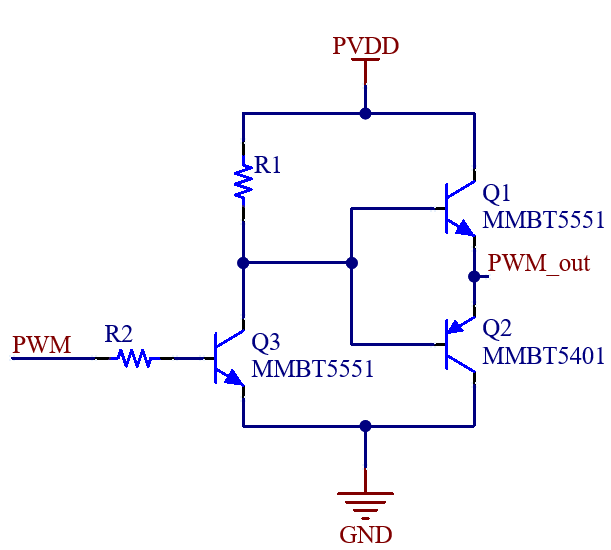
\includegraphics[scale=0.5]{imagenes/clk_gen.png}
        \caption{Inversor utilizado para generar la señal cuadrada}
        \label{fig:inversor}
    \end{figure}

    Para determinar los valores de $R_1$ y $R_2$
    se asumió que el voltaje entre base y emisor ($v_{be}$) del transistor $Q_3$
    es de $1\text{V}$  y que la ganancia en corriente del 
    transistor $Q_3$ es de $10$ \cite{mmtb5551}. Con lo anterior, se fijó el 
    valor de $R_2$ en $1\text{K}\Omega$, por 
    lo que la corriente en la base de $Q_3$ es de $I_b = 4\text{mA}$, y el valor
     esperado para la corriente de colector es de $I_c = 40\text{mA}$.

    Para que este transistor actúe como un inversor es necesario que 
    el transistor $Q_3$ se encuentre alternando entre
    las regiones de corte y saturación. Para ello es necesario
    que el producto $I_cR_1$ sea mayor al voltaje en el nodo PVDD, el cual
    es de $12\text{V}$:
    
    $$
        I_cR_1 > 12\text{V}
    $$
    
   
    $$
        R_1 > \frac{12\text{V}}{40\text{mA}} = 300 \Omega
    $$

    
    Por lo que se utilizó un valor de $R_1 = 1\text{K}\Omega$. Esta señal es 
    pasada en la etapa \textit{push-pull} para aumentar la corriente de salida
    del inversor,asi como disminuir la impedancia, de forma que sea 
    capaz de alimentar el multiplicador de voltaje.

    Para el diseño del multiplicador de voltaje se estableció que la 
    el valor de $C_1$ y $C_2$ sea de
    $1\mu\text{F}$, que el valor de salida requerido debe ser menor o igual
    a $-7\text{V}$ y el número de etapas($N$) es igual a 1. En la 
    ecuación \ref{eq:dickson_charge_neg}  se toma en cuenta la
    capacitancia parásita de los diodos ($C_s$), para el diseño se asumió
    que estas capacitancias no son significativas en comparación con 
    $C_1$ y $C_2$,por lo que se asume $C_s = 0$.
    Con lo anterior, la ecuación \ref{eq:charge_pump} se simplifica a la
    ecuación \ref{eq:charge_pump_simp}. En la figura \ref{fig:charge_pump_dis}
    se muestra el circuito diseñado.

    \begin{figure}[H]
        \centering
        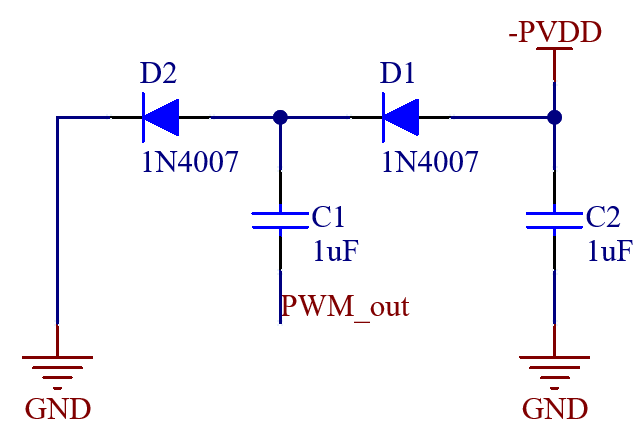
\includegraphics[scale=0.5]{imagenes/dickson_charge.png}
        \caption{Circuito diseñado para el multiplicador de voltaje}
        \label{fig:charge_pump_dis}
    \end{figure}

    \begin{equation}
        V_{out} = -\left(V_\Phi - V_D - \frac{I_{out}}{Cf}  \right)
        \label{eq:charge_pump_simp}
    \end{equation}

    Para determinar la frecuencia de operación, se utilizó la ecuación 
    \ref{eq:charge_pump_simp}, junto con la desigualdad 
    $V_{out} \leq -7\text{V}$, obteniendo la ecuación 
    \ref{eq:charge_pump_simp2}.

    \begin{equation}
        -\left(V_\Phi - V_D - \frac{I_{out}}{Cf}\right) \leq -7\text{V}
        \label{eq:charge_pump_simp2}    
    \end{equation}

    Para la amplitud de la señal cuadrada se utilizó el valor de 
    $V_\Phi = 12 \text{V}$, mientras que para 
    el valor de $V_D$ se utilizó el valor de $0.7\text{V}$, y se estimó que
    la corriente de salida del multiplicador de voltaje es de $10\text{mA}$.
    Despejando para la frecuencia se obtiene la ecuación \ref{eq:charge_pump_simp3}.

    \begin{equation}
        f \geq \frac{I_{out}}{C(V_\Phi - V_D - V_{out})}
        \label{eq:charge_pump_simp3}
    \end{equation}

    Reemplazando los valores en la ecuación \ref{eq:charge_pump_simp3} se obtiene
    la frecuencia de operación del multiplicador de voltaje debe de ser 

        $$
            f \geq \frac{10\text{mA}}{1\mu\text{F}(12\text{V} - 0.7\text{V}
             - 7\text{V})} \approx 2.325\text{KHz}
        $$

    Ya que este es un valor mínimo para la frecuencia de operación, al utilizar
    una frecuencia mayor se obtendrá un voltaje de salida mayor, por lo que se
    utilizó una frecuencia de operación de $7.81\text{KHz}$, la cual es la
    frecuencia de la señal PWM generada por el microcontrolador. 
